\chapter{Acoustic Pulse Recognition System}\label{ch:APR}

\ifpdf
    \graphicspath{{Chapter3_APR/Chapter3Figs/PNG/}{Chapter3_APR/Chapter3Figs/PDF/}{Chapter3_APR/Chapter3Figs/}}
\else
    \graphicspath{{Chapter3_APR/Chapter3Figs/EPS/}{Chapter3_APR/Chapter3Figs/}}
\fi

This chapter describes work undertaken with several waveform classification algorithms, specifically designed to detect and classify taps incident on a device containing a single microphone. The different models in the classification algorithms correspond to different tapping positions $j$ on the device, and the algorithms can therefore be said to represent a new touch screen technology using Acoustic Pulse Recognition (APR). This chapter is specifically focussed on applications using a single sensor to attempt to tackle the difficult issue of the structural uncertainty and its effect on recorded waveforms without the aid of inter microphone time and intensity differences.

Traditionally the given data in selection problems have been referred to as models. In the following section these models will occasionally be referred to as templates in the context of the specific models for this application.

\section{Background}
Modern touch screen devices have, generally speaking, 2 main attributes. Firstly they function without the need for any additional interfacing hardware and secondly they let a user interact directly with the data presented to the user. The methods introduced in the following sections attempts to reconcile these attributes with factors such as scalable deployment and low manufacturing and implementation costs through APR.

The underlying assumption of an APR system is that tapping on any spot, on the touch sensitive surface, creates a unique acoustical pulse, that this unique pulse is largely reproducible and that it is detectable. Figure~\ref{fig:twotwoSampleTap} shows a plot of 4 tap pulses recorded at 2 different spots on the device. It is seen from the plot that tapping in these two different locations produce noticeably different pulses and that the pulses from the same spot is, though slightly different in certain parts of the signal, still visibly similar. The 4 taps in Figure~\ref{fig:twotwoSampleTap} have been aligned to the onset of the tap.

\begin{figure}[t]
  \begin{center}
    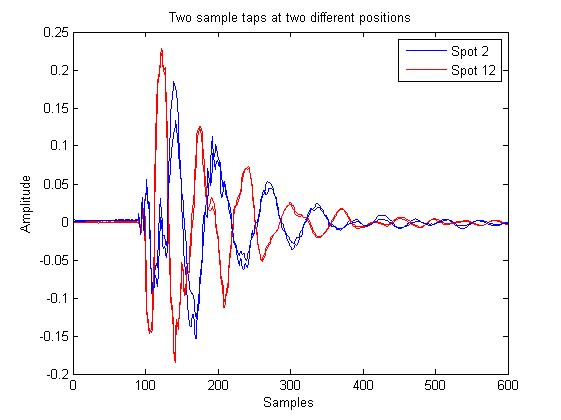
\includegraphics[width=110mm]{twotwoSampleTap}
    \caption{Two taps recorded at both spot 1 and 12. Sampled at 44.1 kHz.}\label{fig:twotwoSampleTap}
  \end{center}
\end{figure}

%Maybe not use this paragraph... rewrite at least.
Although Figure~\ref{fig:twotwoSampleTap} shows the scope of the variability in the pulses due to impact site, it is worth recognizing that this variability is fairly modest compared to the variability observed when comparing tapping pulses with data such as speech or even other percussive signals. It is also worth noting that some variability arises from certain environmental conditions, so the nature of the problem can be summed up as being one where certain variations are expected and others are used as the basis for classification.

\section{System}\label{sec:APRsystem}
The system developed consists of a number of different elements that crudely can be divided into hardware and software. The hardware system can be considered as a testing rig for the algorithm and is designed to facilitate a single output black box type approach to the classification problem, where the black box represents a unknown complex vibrational system with certain transfer characteristics. These characteristics are assumed to be reproducible or time-invariant. Figure~\ref{fig:blackBox} represents such a system,

\begin{figure}[!]
\centering
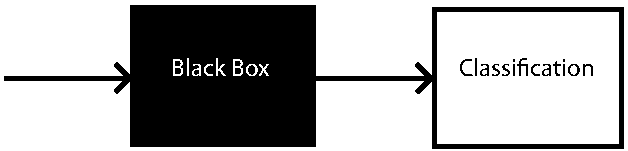
\includegraphics[width=100mm]{blackBox.pdf}
\caption{Black box representation of structural uncertainty in a tapping device.}\label{fig:blackBox}
\begin{picture}(0,0)
\put(-120,83){$x^j$}
\put(22,83){$y$}
\end{picture}
\end{figure}

where $x^j$ can be considered some pulse on a spot $j$ known by the user, while $y$ is the output of the black box as seen by the classification algorithm oblivious to the origin of the tap $j$.

Two pieces of hardware were produced to achieve these characteristics. Firstly a mobile phone implementation of the algorithm was considered and an actual mobile phone handset was acquired and modified to allow for external analogue monitoring of the internal microphone. The mobile phone chosen for this application was a Samsung SGH-M150, which can be seen in Figure~\ref{fig:phone}. This device was chosen based on its ability to be easily modified to allow for external interfacing the microphone. Additionally a grid of $J = 12$ points was added to the screen area as reference points for tapping.

\begin{figure}[!]
\centering
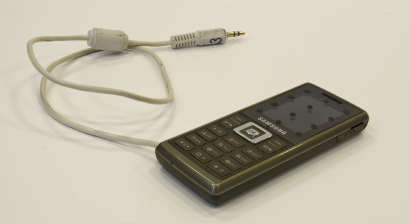
\includegraphics[width=410 px]{phone.png}
\caption{Picture of modified Samsung SGH-M150 mobile phone with 12 spot grid on display area.}\label{fig:phone}
\end{figure}

A larger application of the same black box characteristics is a simple wooden board, measuring $30.6 \times 24.3 \times 1.8$ cm (l$\times$w$\times$d), with a grid of 30 spots marked on the face of it. Attached on the back of the board, in a small cavity, is a microphone to pick up an acoustic signal from the board when tapped.  The board can be seen in Figure~\ref{fig:Pad}. The microphone used for this application is a DPA Microphone 4060 omnidirectional condenser microphone. This microphone was chosen for its excellent linear characteristics, its high sensitivity and dynamic range.

\begin{figure}[!]
\centering
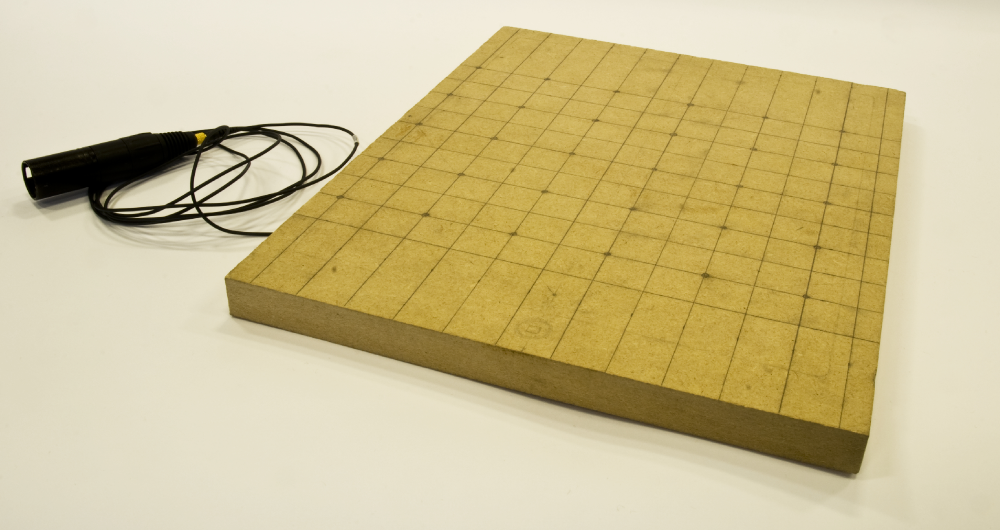
\includegraphics[width=410 px]{Pad.png}
\caption{Picture of wooden board with attached microphone to the back and 30 spot grid on the front.}\label{fig:Pad}
\end{figure}

The second part of the system is the software. Figure~\ref{fig:system} shows a simple block diagram representing the system where the bottom row is meant to represent the software system. The display on this figure represents the output from the interpolation extension to the ML and MAP methods, described later in the chapter. In this system definition, the hardware can be viewed as being the ``restricting'' factor while the software is the ``redeeming'' factor, and hence the attention is now turned to the models and algorithms of the system.

\begin{figure}[!htbp]
  \centering
    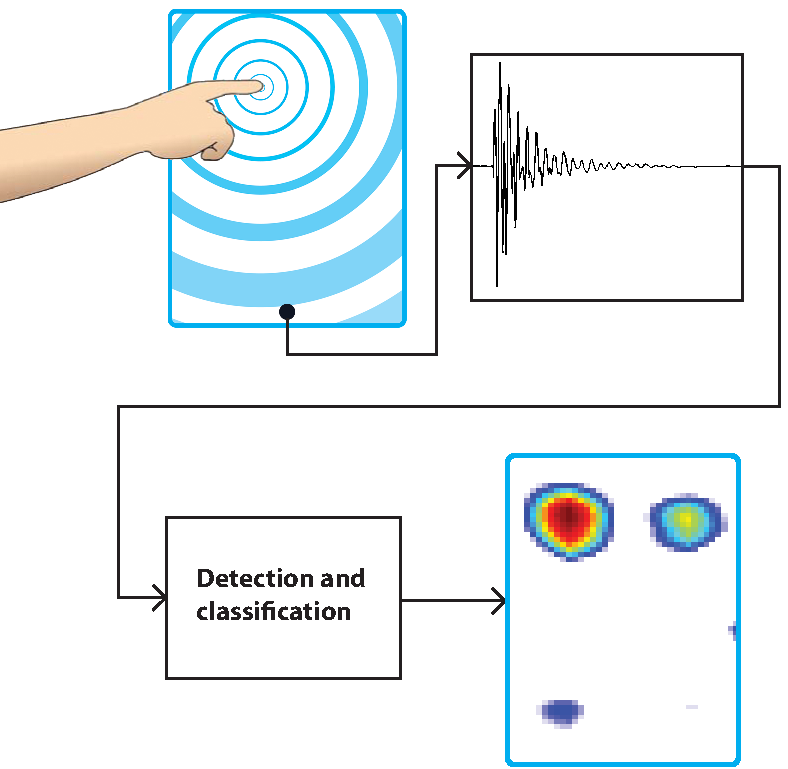
\includegraphics[width=110mm]{system.pdf}
    \caption{Block diagram of detection system. The display displays an intensity map of likelihoods superimposed on the device, as described in the extension to the ML and MAP methods.}\label{fig:system}
\begin{picture}(0,0)
\put(-136,226){Microphone}
\put(-57,166){DSP}
\put(72,191){Display}
\put(50,351){Tapping pulse}
\put(-72,230){\vector(2,1){25}}
\end{picture}
\end{figure}

\section{ML and MAP methods}
\subsection{Model and theory}
Suppose that each data reading $y = [y_0, \ldots , y_{N-1}]^T $ is modeled by the linear model

\begin{equation}\label{eq:MLmod1}
y = \theta^j t^j(n_0) + v,
\end{equation}

where $t$ is a set of $J$ templates from $J$ different spots so that $t^j(n_0)$ is then the $j$th template, $j \in \{1, \ldots ,J\}$ shifted to time $n_0$ and $\theta$ is taken to be a random variable describing the scaling of the template.

\begin{equation}\label{eq:MLtheta}
\theta \sim \mathcal{N}(\mu_{\theta},\sigma_{\theta}^2),
\end{equation}

where $v$ is the independent and identically distributed (i.i.d.) Gaussian noise, modeling the background interference.

\begin{equation}\label{eq:MLnoise}
v_n \stackrel{i.i.d.}{\sim} \mathcal{N}(0,\sigma_{v,n}^2).
\end{equation}

To evaluate which, if any, of the templates that are present in the data and when they are observed we need to evaluate the probability of the template number $j$ and the time shift $n_0$ given the received data $y$ which can be described as $p(j,n_0|y)$.

Using Bayes' theorem it is found that:

\begin{equation}\label{eq:MLBayes}
p(j,n_0|y) \propto p(y|j,n_0)p(j,n_0),
\end{equation}

where $p(j,n_0|y)$ is the posterior probability, $p(y|j,n_0)$ is the likelihood and $p(j,n_0)$ is the prior probability.
Take the prior probability to be:

\begin{equation}\label{eq:MLPrior}
p(j,n_0) = \frac{1}{JN},
\end{equation}
as the expression for a non-informative prior. This ignorant prior can be modified with time.
The likelihood can be expressed as the marginalization of the conditional probability of the data $y$ given the scaling $\theta$, template number $j$ and the time shift $n_0$, over $\theta$, so that:

\begin{equation}\label{eq:MLmargin}
p(y|j,n_0)=\int_\theta p(y|\theta, j, n_0) p(\theta) d\theta,
\end{equation}

where the product of the two normal distributions $p(y|\theta, j, n_0)$ and $p(\theta)$, can be expressed as a third unnormalized normal distribution and a normalizing constant $z$.

\begin{equation}\label{eq:MLprod1}
\mathcal{N}_y(\theta t^j(n_0),\sigma_v^2)\cdot\mathcal{N}_\theta(\mu_\theta,\sigma^2_\theta) = z \times \mathcal{N}_\theta(\hat{\mu}_\theta,\hat{\sigma}^2_\theta),
\end{equation}
where $\mathcal{N}_\theta(\hat{\mu}_\theta,\hat{\sigma}_\theta^2)$ is the third normal distribution which is the only element on the r.h.s. which is dependent on $\theta$,

\begin{equation}\label{eq:MLtheta2}
\mathcal{N}_\theta(\mu_\theta,\sigma^2_\theta) = \frac{1}{\sqrt{2 \pi \sigma_\theta^2}} \textrm{exp}\left[-\frac{\left(\theta - \mu_\theta\right)^2}{2\sigma_\theta^2}\right],
\end{equation}

and

\begin{equation}\label{eq:MLnoise2}
\mathcal{N}_y(\theta t^j(n_0),\sigma_v^2) = \frac{1}{\sqrt{2 \pi \sigma_v^2}} \textrm{exp}\left[-\frac{\left(y - \theta t^j\left(n_0\right)\right)^2}{2\sigma_v^2}\right].
\end{equation}

It is now possible to write the marginalization in equation (\ref{eq:MLmargin}) as:

\begin{equation}\label{eq:MLmargin2}
p(y|j,n_0)=\int_\theta \mathcal{N}_y(\theta t^j(n_0),\sigma_v^2)\cdot\mathcal{N}_\theta(\mu_\theta,\sigma^2_\theta) d\theta = z \int_\theta \mathcal{N}_\theta(\hat{\mu}_\theta,\hat{\sigma}^2_\theta) d\theta = z,
\end{equation}

since $\int_\theta \mathcal{N}_\theta(\hat{\mu}_\theta,\hat{\sigma}^2_\theta) d\theta = 1$.

To evaluate $\hat{\sigma}^2_\theta$ and $\hat{\mu}_\theta$, the l.h.s. of equation (\ref{eq:MLprod1}) must be expanded,

\begin{eqnarray}\label{eq:MLprod3}
& & \mathcal{N}_y(\theta t^j(n_0),\sigma_v^2)\cdot\mathcal{N}_\Theta(\mu_\theta,\sigma^2_\theta) \\\nonumber{}\\\nonumber
& & \quad = \frac{1}{2\pi \sigma_v \sigma_\theta} \textrm{exp}\left[-\frac{1}{2}\left(\frac{y^Ty +\theta^2t^j(n_0)^Tt^j(n_0)-2\theta y^T t^j(n_0)}{\sigma^2_v}+\frac{\theta^2 + \mu^2_\theta-2\theta\mu_\theta}{\sigma_\theta^2}\right)\right]\\\nonumber{}\\\nonumber
& & \quad = \frac{1}{2\pi \sigma_v \sigma_\theta} \textrm{exp}\left[-\frac{1}{2}\left(\theta^2 \left(\frac{1}{\sigma_\theta^2}+\frac{t^j(n_0)^T t^j(n_0)}{\sigma_v^2}\right) - 2\theta\left(\frac{y^T t^j(n_0)}{\sigma_v^2}+\frac{\mu_\theta}{\sigma_\theta^2}\right) + \frac{y^Ty}{\sigma_v^2} +\frac{\mu_\theta^2}{\sigma_\theta^2}\right)\right].
\end{eqnarray}

Expanding the r.h.s. of equation (\ref{eq:MLprod1}) gives

\begin{eqnarray}\label{eq:MLprod4}
& & z \times \mathcal{N}_\theta(\hat{\mu}_\theta,\hat{\sigma}^2_\theta) \\\nonumber{}\\\nonumber
& & \quad = \frac{z}{\sqrt{2 \pi}\hat{\sigma}_\theta}\textrm{exp}\left[-\frac{1}{2}\left(\theta^2\frac{1}{\hat{\sigma}^2_\theta} - 2\theta\frac{\hat{\mu}_\theta}{\hat{\sigma}^2_\theta} + \frac{\hat{\mu}_\theta^2}{\hat{\sigma}^2_\theta}  \right)\right]
\end{eqnarray}

By observation between equation (\ref{eq:MLprod3}) and (\ref{eq:MLprod4}) it is found that:

\begin{eqnarray}
\label{eq:MLprod5}
\hat{\sigma}^2_\theta &=& \left(\frac{t^j(n_0)^T t^j(n_0)}{\sigma_v^2} + \frac{1}{\sigma_\theta^2}\right)^{-1} \qquad \textrm{and}\\\nonumber
\hat{\mu}_\theta &=& \left(\frac{y^T t^j(n_0)}{\sigma_v^2} + \frac{\mu_\theta}{\sigma^2_\theta}\right)\hat{\sigma}^2_\theta.
\end{eqnarray}

From equation (\ref{eq:MLprod1}) we have that,

\begin{equation}\label{eq:MLprod2}
z = \frac{\mathcal{N}_y(\theta t^j,\sigma_v^2)\cdot\mathcal{N}_\Theta(\mu_\theta,\sigma^2_\theta)}{\mathcal{N}_\theta(\hat{\mu}_\theta,\hat{\sigma}^2_\theta)}
\end{equation}

and substituting in equation (\ref{eq:MLprod3}) and (\ref{eq:MLprod4}):

\begin{eqnarray}\label{eq:MLprod6}
z &=& \frac{\frac{1}{2\pi \sigma_v \sigma_\theta} \textrm{exp}\left[-\frac{1}{2}\left(\theta^2 \left(\frac{1}{\sigma_\theta^2}+\frac{t^j(n_0)^T t^j(n_0)}{\sigma_v^2}\right) - 2\theta\left(\frac{y^T t^j(n_0)}{\sigma_v^2}+\frac{\mu_\theta}{\sigma_\theta^2}\right) + \frac{y^T y}{\sigma_v^2} +\frac{\mu_\theta^2}{\sigma_\theta^2}\right)\right]}{\frac{1}{\sqrt{2 \pi}\hat{\sigma}_\theta}\textrm{exp}\left[-\frac{1}{2}\left(\theta^2\frac{1}{\hat{\sigma}^2_\theta} - 2\theta\frac{\hat{\mu}_\theta}{\hat{\sigma}^2_\theta} + \frac{\hat{\mu}_\theta^2}{\hat{\sigma}^2_\theta}  \right)\right]}.
\end{eqnarray}

Substituting in values for $\hat{\sigma}^2_\theta$ and $\hat{\mu}_\theta$ from equation (\ref{eq:MLprod5}), and with a bit of rewriting equation (\ref{eq:MLprod6}) reduces to:

\begin{equation}\label{eq:MLprod7}
z = \frac{1}{\sqrt{2 \pi}\phi \sigma_v \sigma_\theta}\textrm{exp}\left[-\frac{1}{2}\left(\frac{y^T y}{\sigma^2_v}+\frac{\mu_\theta^2}{\sigma_\theta^2} - \frac{\left(\frac{y^T t^j(n_0)}{\sigma_v^2}+\frac{\mu_\theta}{\sigma_\theta^2}\right)^2}{\phi}\right)\right],
\end{equation}

where $\phi = \hat{\sigma}^{-2}_\theta = \frac{t^j(n_0)^Tt^j(n_0)}{\sigma_v^2} + \frac{1}{\sigma_\theta^2}$. Remembering equation (\ref{eq:MLmargin2}) where $p(y|j,n_0) = z$ the probability of the data $y$ conditional on the model $j$ and the time shift $n_0$ is now known and can be referred to as the likelihood of the model $j$. An estimate of the model present in the data can be found by inspecting the likelihood function over the range of models. This method is called the Maximum Likelihood estimate or ML estimate, and is given by:

\begin{equation}\label{eq:MLdefinition}
j_{ML} = \arg\max_j p(y|j,n_0).
\end{equation}

It is often useful to consider the log-likelihood rather than the likelihood due to computational complexity inherent in the exponential function. It is worth noting that the log-likelihood and the likelihood gives the same estimate since log is a monotonic transformation.

The log-likelihood is found to be:

\begin{equation}\label{eq:MLloglikelihood}
\log{p(y|j,n_0)} = -\frac{\log{2\pi}}{2} - \log{\phi} - \log{\sigma_v} -\log{\sigma_\theta} - \frac{y^T y}{2\sigma_v^2} -\frac{\mu^2_\theta}{2\sigma^2_\theta} + \frac{\left(\frac{y^T t^j(n_0)}{\sigma^2_v}-\frac{\mu_\theta}{\sigma^2_\theta}\right)^2}{2\phi},
\end{equation}

where several other monotonic elements can be eliminated for simplicity.

Another useful statistic to consider is the Maximum \emph{A Posterior} (MAP) estimate of the model $j$. The MAP estimate is given by:

\begin{equation}\label{eq:MAPdefinition}
j_{MAP} = \arg\max_j p(y|j,n_0)p(j,n_0).
\end{equation}


\section{PCA type method}\label{sec:APRpca}
While the ML and MAP methods provide a simple and reasonably effective model selection algorithm, a range of environmental factors can have an impact on the recorded pulse. Figure~\ref{fig:shiftOverTemperature} shows 6 different mean templates recorded at 6 different temperatures in the range of 19.5 to 34.4 $^o$C.

\begin{figure}[!]
\centering
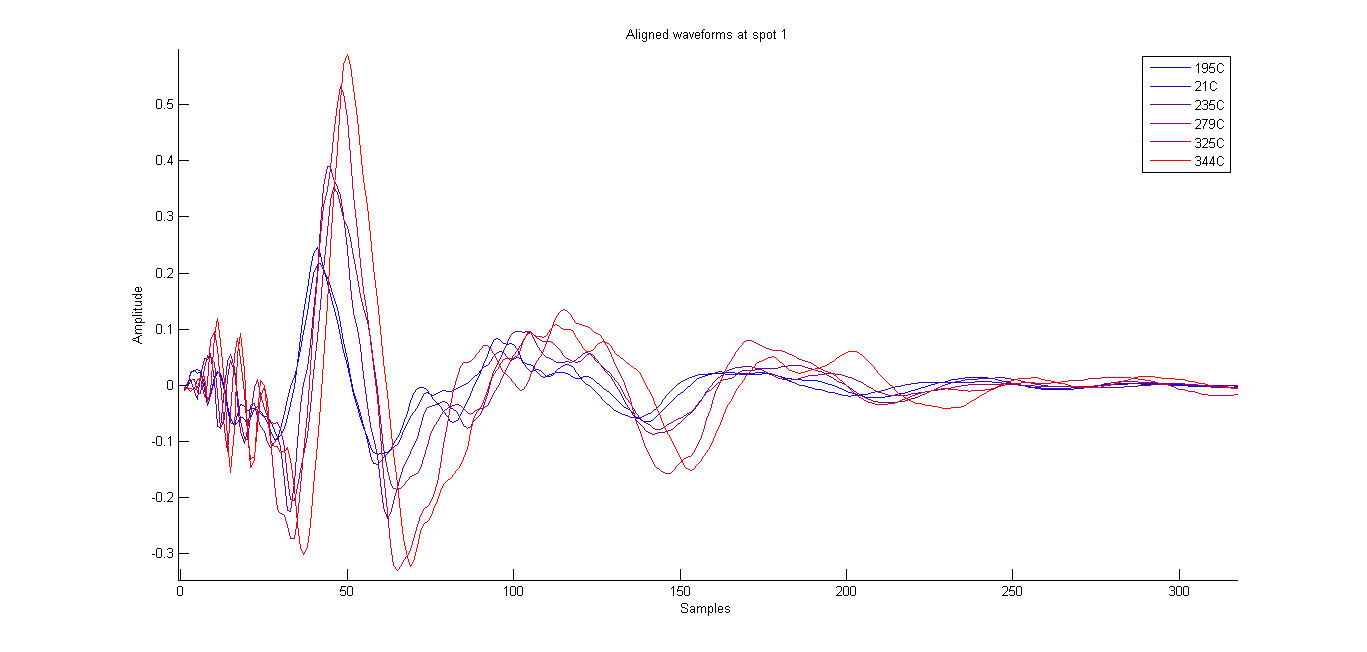
\includegraphics[width=150mm]{shiftOverTemperature.png}
\caption{6 different mean templates trained a 6 different temperatures on the same spot. Sampled at 44.1 kHz and aligned.}\label{fig:shiftOverTemperature}
\end{figure}
It appears that the temperature has a dramatic effect on the mean template and as such it seems questionable whether or not the previously described ML and MAP method would be able to cope with this level of variation. Pulse variability has also been detected when users hold the devices in different ways, have the device on a surface and tap with nails or different styluses. The PCA type method is an attempt at singling out significant components of the pulse that relate to the tapping position rather than the other factors mentioned above, and to record the variability within the significant components.

\begin{figure}[!]
\centering
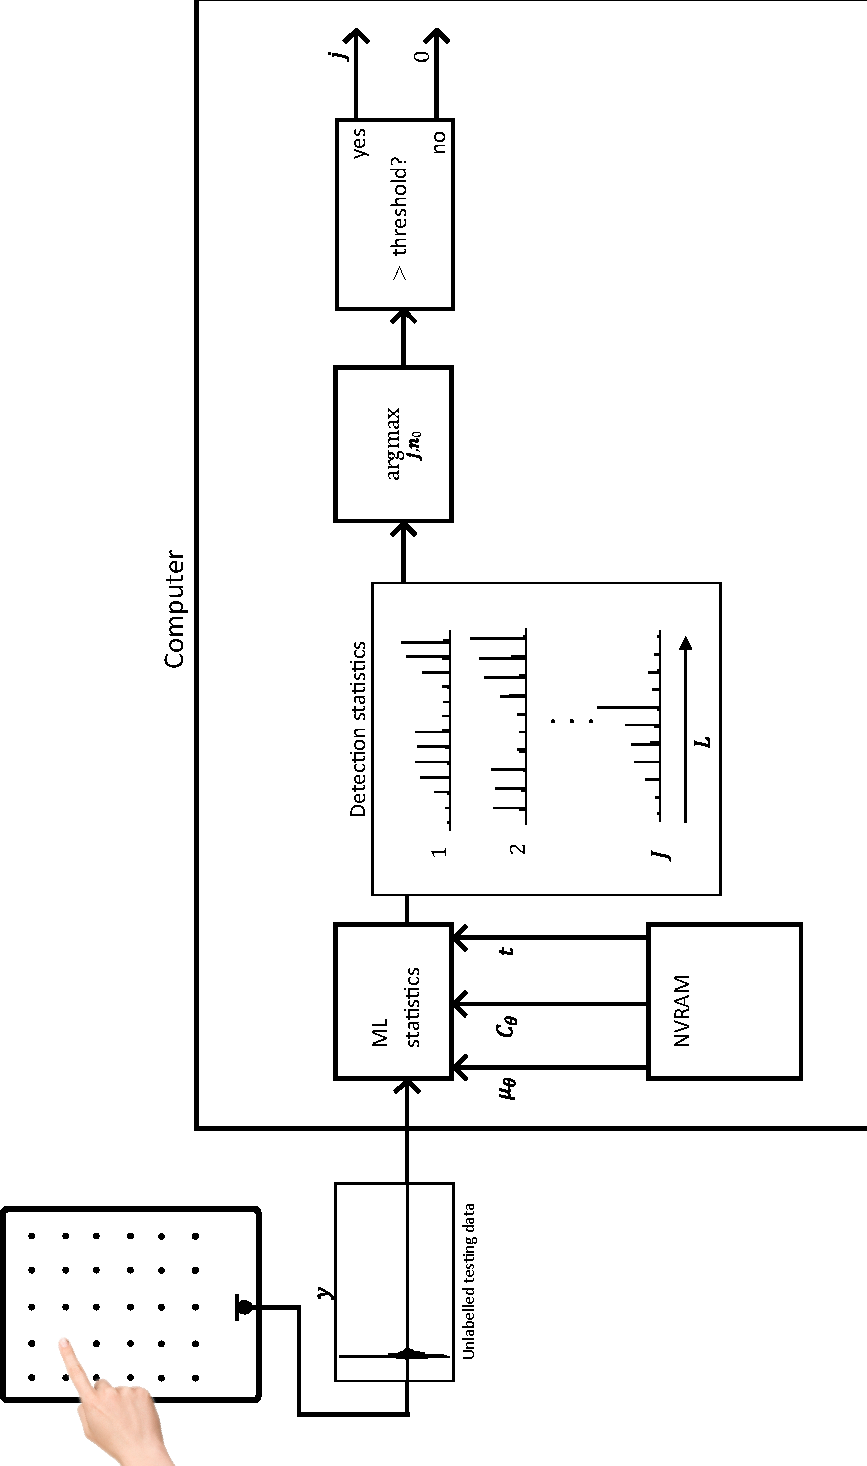
\includegraphics[width=360px]{testingSystemPlot.pdf}
\caption{Block diagram of detection/use stage of algorithm.}\label{fig:testingSystemPlot}
\end{figure}

Figure~\ref{fig:testingSystemPlot} shows a block diagram of the implementation of the use/testing stage of the algorithm. The diagram shows how a tap $y$ incident on the tapping device is picked up by the microphone on the device and transmitted to a computer. Within the computer the algorithm calculates the statistics, as outlined below, utilizing data from the training stage of the algorithm. The statistics of the signal is then evaluated and the most probable class or spot is displayed to the user unless the models do not yield a sufficiently high probability, as determined by a threshold, in which case no tap will be registered.

\subsection{Model and theory}
A standard linear instantaneous model is considered where observations $y = [y_0, \ldots , y_{N-1}]^T $ are modeled as a noisy linear combination:

\begin{equation}\label{eq:mod1}
y = \sum_{i=1}^{I} \theta_i^j t_i^j(n_0) + v,
\end{equation}

where $t_i^j(n_0)$ is the $j$th template, $j \in \{1, \ldots ,J\}$, for $I$ independent components and $\theta_i^j$ is the amplitude of the $j$th spot and $i$th component. In this section the model has been assumed to be of zero mean $\mu^j(n_0) =0$ although this assumption could easily be avoided by adding it to the model. Take $\theta_i^j$ to be a random variable, $\Theta^j = [\theta_1^j,\ldots,\theta_I^j]^T$, describing the scale of each template component $i$ where

\begin{equation}\label{eq:theta}
\Theta^j \sim \mathcal{N}(\mu_{\Theta}^j,C_{\Theta}^j),
\end{equation}

and Gaussian noise to model background interference:

\begin{equation}\label{eq:noise}
v_n \stackrel{i.i.d.}{\sim} \mathcal{N}(0,\sigma_{v,n}^2).
\end{equation}

Considering this model in matrix notation:
\begin{equation}\label{eq:mod2}
y = \textbf{t}\Theta + \textbf{v}.
\end{equation}

For simplicity the matrices $\textbf{t}^j(n_0)$ and $\Theta^j$ will from now on be referred to as simply $\textbf{t}$ and $\Theta$ respectively.
Bayes' theorem can now be used to evaluate the joint probability of $y$ and $\Theta$ as

\begin{equation}\label{eq:bayes1}
p(y,\Theta | j) = p(y|\Theta,j)p(\Theta | j).
\end{equation}

Since the goal is to evaluate the probability of each data reading $y$ given a particular position/model $j$, the dependency of $\Theta$ can be marginalized out,

\begin{eqnarray}\nonumber
p(y|j) &=& \int_\Theta p(y,\Theta|j) d\Theta \\
\label{eq:marg1} &=& \int_\Theta p(y|\Theta,j)p(\Theta|j) d\Theta.
\end{eqnarray}

Given (\ref{eq:noise}) and (\ref{eq:mod2}), the probability $p(y|\Theta)$ can be expressed as:

\begin{equation}\label{eq:probybeta}
p(y|\Theta,j) = \mathcal{N}_y(\textbf{t}\Theta,\sigma_v^2\textbf{I}),
\end{equation}
where $\textbf{I}$ is the identity matrix.
Now (\ref{eq:marg1}) can be written as:

\begin{equation}\label{eq:marg2}
p(y|j) = \int_\Theta \mathcal{N}_y(\textbf{t}\Theta,\sigma_v^2 \textbf{I})\times\mathcal{N}_\Theta(\mu_\Theta,C_\Theta) d\Theta
\end{equation}

The product of two normal distributions is another normal distribution and since this resulting normal distribution is no longer normalized a normalizing constant $z$ is added:

\begin{equation}\label{eq:prod1}
\mathcal{N}_y(\textbf{t}\Theta,\sigma_v^2 \textbf{I})\cdot\mathcal{N}_\Theta(\mu_\Theta,C_\Theta) = z \times \mathcal{N}_\Theta(\hat{C}_\Theta,\hat{\mu}_\Theta)
\end{equation}

Since:
\begin{equation}\label{eq:marg3}
\int_\Theta \mathcal{N}_\Theta(\hat{C}_\Theta,\hat{\mu}_\Theta) d\Theta = 1,
\end{equation}
we have that:
\begin{equation}\label{eq:marg4}
p(y|j) = z \times \int_\Theta \mathcal{N}_\Theta(\hat{C}_\Theta,\hat{\mu}_\Theta) d\Theta = z.
\end{equation}

To evaluate $z$ the l.h.s. of equation (\ref{eq:prod1}) is expanded
{\setlength\arraycolsep{2pt}
\begin{eqnarray}
\label{eq:prod2} & & \mathcal{N}_y(\textbf{t}\Theta,\sigma_v^2 \textbf{I})\times\mathcal{N}_\Theta(\mu_\Theta,C_\Theta) = \\\nonumber
& & \qquad \frac{1}{(2\pi)^{\frac{n}{2}} |\sigma_v^2\textbf{I}|^{\frac{1}{2}}} \textrm{exp}\left[-\frac{1}{2}(y - \textbf{t}\Theta)^T(\sigma_v^2 \textbf{I})^{-1}(y - \textbf{t}\Theta)\right] \times {} \\\nonumber
& & \qquad \frac{1}{(2\pi)^{\frac{n}{2}}|C_\Theta|^{\frac{1}{2}}} \textrm{exp}\left[-\frac{1}{2}(\Theta - \mu_\Theta)^TC_\Theta^{-1}(\Theta - \mu_\Theta)\right] \\\nonumber
& & \quad= \frac{1}{(2\pi)^n |\sigma_v^2\textbf{I}|^{\frac{1}{2}} |C_\Theta|^{\frac{1}{2}}} \textrm{exp}\bigg[-\frac{\textbf{I}}{2\sigma_v^2}\left(y^Ty+\Theta^T\textbf{t}^T\textbf{t}\Theta - 2 \Theta^T\textbf{t}y\right) - {} \\\nonumber
& & \qquad \frac{1}{2C_\Theta} \left(\Theta^T\Theta + \mu_\Theta^T\mu_\Theta - 2 \Theta^T\mu_\Theta\right) \bigg] \\\nonumber
& & \quad = \frac{1}{(2\pi)^n |\sigma_v^2\textbf{I}|^{\frac{1}{2}} |C_\Theta|^{\frac{1}{2}}} \textrm{exp}\Bigg[-\frac{1}{2}\Bigg(\Theta^T\left(\frac{\textbf{t}^T\textbf{t}}{\sigma_v^2} + C_\Theta^{-1}\right)\Theta - 2 \Theta^T\left(\frac{\textbf{t}y}{\sigma_v^2} + \frac{\mu_\Theta}{C_\Theta}\right) + {}\\\nonumber
& & \qquad \mu_\Theta^TC_\Theta^{-1}\mu_\Theta + \frac{y^Ty}{\sigma_v^2}\Bigg)\Bigg].
\end{eqnarray}}
The r.h.s. of equation (\ref{eq:prod1}) is also expanded,

{\setlength\arraycolsep{2pt}
\begin{eqnarray}
\label{eq:prod3} & & z \times \mathcal{N}_\Theta(\hat{C}_\Theta,\hat{\mu}_\Theta) \\\nonumber
& & \quad = z\frac{1}{(2\pi)^{\frac{n}{2}} |\hat{C}_\Theta|^{\frac{1}{2}}} \textrm{exp}\left[-\frac{1}{2}\left(\Theta - \hat{\mu}_\Theta\right)^T\hat{C}_\Theta^{-1}\left(\Theta - \hat{\mu}_\Theta\right)\right] \\\nonumber
& & \quad = z\frac{1}{(2\pi)^{\frac{n}{2}} |\hat{C}_\Theta|^{\frac{1}{2}}} \textrm{exp}\left[-\frac{1}{2}\left(\Theta^T\hat{C}_\Theta^{-1}\Theta + \hat{\mu}_\Theta^T\hat{C}_\Theta^{-1}\hat{\mu}_\Theta - 2\Theta^T\hat{C}_\Theta^{-1}\hat{\mu}_\Theta\right)\right],
\end{eqnarray}}
and by inspection and comparison between equation (\ref{eq:prod2}) and (\ref{eq:prod3}) it is found that:

\begin{eqnarray}
\label{eq:prod4}
\hat{C}_\Theta &=& \left(\frac{\textbf{t}^T\textbf{t}}{\sigma_v^2} + C_\Theta^{-1}\right)^{-1} \qquad \textrm{and}\\\nonumber
\hat{\mu}_\Theta &=& \left(\frac{\textbf{t}^Ty}{\sigma_v^2} + \frac{\mu_\Theta}{C_\Theta}\right)\hat{C}_\Theta.
\end{eqnarray}

Equation (\ref{eq:prod2}) and (\ref{eq:prod4}) are equated and the normalizing constant $z$ is isolated.

{\setlength\arraycolsep{2pt}
\begin{eqnarray}\label{eq:z1}
z &=& \frac{(2\pi)^{\frac{n}{2}}\left|\hat{C}_\Theta\right|^{\frac{1}{2}} }{(2\pi)^n |\sigma_v^2\textbf{I}|^{\frac{1}{2}} |C_\Theta|^{\frac{1}{2}}} \times {}\\\nonumber
& &\frac{\textrm{exp}\Bigg[-\frac{1}{2}\Bigg(\Theta^T\left(\frac{\textbf{t}^T\textbf{t}}{\sigma_v^2} + C_\Theta^{-1}\right)\Theta - 2 \Theta^T\left(\frac{\textbf{t}y}{\sigma_v^2} + \frac{\mu_\Theta}{C_\Theta}\right) + \mu_\Theta^TC_\Theta^{-1}\mu_\Theta + \frac{y^Ty}{\sigma_v^2}\Bigg)\Bigg]}{\textrm{exp}\left[-\frac{1}{2}\left(\Theta^T\hat{C}_\Theta^{-1}\Theta - 2\Theta^T\hat{C}_\Theta^{-1}\hat{\mu}_\Theta + \hat{\mu}_\Theta^T\hat{C}_\Theta^{-1}\hat{\mu}_\Theta \right)\right]}.
\end{eqnarray}}
Substituting $\hat{C}_\Theta$ from equation~(\ref{eq:prod4}) and doing some simplification, gives:
{\setlength\arraycolsep{2pt}
\begin{eqnarray}\label{eq:z2}
z &=& \frac{\left|\frac{\textbf{t}^T\textbf{t}}{\sigma_v^2} + C_\Theta^{-1}\right|^{-\frac{1}{2}}}{(2\pi)^{\frac{n}{2}} |\sigma_v^2\textbf{I}|^{\frac{1}{2}} |C_\Theta|^{\frac{1}{2}}} \times {}\\\nonumber
& &\frac{\textrm{exp}\Bigg[-\frac{1}{2}\Bigg(\Theta^T\left(\frac{\textbf{t}^T\textbf{t}}{\sigma_v^2} + C_\Theta^{-1}\right)\Theta - 2 \Theta^T\left(\frac{\textbf{t}y}{\sigma_v^2} + \frac{\mu_\Theta}{C_\Theta}\right) +  \mu_\Theta^TC_\Theta^{-1}\mu_\Theta + \frac{y^Ty}{\sigma_v^2}\Bigg)\Bigg]}{\textrm{exp}\left[-\frac{1}{2}\left(\Theta^T \left(\frac{\textbf{t}^T\textbf{t}}{\sigma_v^2} + C_\Theta^{-1}\right)\Theta  - 2\Theta^T\left(\frac{\textbf{t}^T\textbf{t}}{\sigma_v^2} + C_\Theta^{-1}\right)\hat{\mu}_\Theta  + \hat{\mu}_\Theta^T\left(\frac{\textbf{t}^T\textbf{t}}{\sigma_v^2} + C_\Theta^{-1}\right)\hat{\mu}_\Theta \right)\right]}
\end{eqnarray}}
Substituting $\hat{\mu}_\Theta$ from equation~(\ref{eq:prod4}) and doing some simplification, gives:
{\setlength\arraycolsep{2pt}
\begin{eqnarray}\label{eq:z2}
z &=& \frac{1}{(2\pi)^{\frac{n}{2}} |\textbf{t}^T\textbf{t}+\sigma_v^2C_\Theta^{-1}|^{\frac{1}{2}} |C_\Theta|^{\frac{1}{2}}} \times {}\\\nonumber
& &\frac{\textrm{exp}\Bigg[-\frac{1}{2}\Bigg(- 2 \Theta^T\left(\frac{\textbf{t}y}{\sigma_v^2} + \frac{\mu_\Theta}{C_\Theta}\right) +  \mu_\Theta^TC_\Theta^{-1}\mu_\Theta + \frac{y^Ty}{\sigma_v^2}\Bigg)\Bigg]}{\textrm{exp}\left[-\frac{1}{2}\left(- 2\Theta^T\left(\frac{\textbf{t}^Ty}{\sigma_v^2} + \frac{\mu_\Theta}{C_\Theta}\right)  + \left(\left(\frac{\textbf{t}^T\textbf{t}}{\sigma_v^2} + C_\Theta^{-1}\right)^T\right)^{-1}\left(\frac{\textbf{t}^Ty}{\sigma_v^2} + \frac{\mu_\Theta}{C_\Theta}\right)^T\left(\frac{\textbf{t}^Ty}{\sigma_v^2} + \frac{\mu_\Theta}{C_\Theta}\right) \right)\right]}\\\nonumber{}\\\nonumber
&=& \frac{1}{(2\pi)^{\frac{n}{2}} |\Phi|^{\frac{1}{2}} |C_\Theta|^{\frac{1}{2}}}\times \frac{\textrm{exp}\left[-\frac{1}{2\sigma_v^2}\left(\sigma_v^2\mu_\Theta^TC_\Theta^{-1}\mu_\Theta + y^Ty\right)\right]}{\textrm{exp}\left[-\frac{1}{2\sigma_v^2}\left(\left(\Phi^T\right)^{-1}\Lambda^T\Lambda \right)\right]}\\\nonumber{}\\\nonumber
&=& \frac{1}{(2\pi)^{\frac{n}{2}} |\Phi|^{\frac{1}{2}}|C_\Theta|^{\frac{1}{2}}} \textrm{exp}\left[-\frac{1}{2\sigma_v^2}\left(\sigma_v^2\mu_\Theta^TC_\Theta^{-1}\mu_\Theta + y^Ty- \left(\Phi^T\right)^{-1}\Lambda^T\Lambda\right)\right],
\end{eqnarray}}
where:
\begin{eqnarray}
\label{eq:z3}
\Phi &=& \textbf{t}^T\textbf{t} + \sigma_v^2C_\Theta^{-1} \qquad \textrm{and}\\\nonumber
\Lambda &=& \textbf{t}^Ty + \sigma_v^2\mu_\Theta C_\Theta^{-1}.
\end{eqnarray}

As with the previous method, the log-likelihood is calculated

\begin{equation}\label{eq:loglikeli}
\log{p(y|j)} = - \frac{n}{2}\log{2 \pi}- \frac{1}{2}\log{|\Phi|} - \frac{1}{2}\log{|C_\Theta|} - \frac{1}{2\sigma^2_v}\left(\sigma_v^2\mu_\Theta^TC_\Theta^{-1}\mu_\Theta + y^Ty- \left(\Phi^T\right)^{-1}\Lambda^T\Lambda\right)
\end{equation}

and maximized over the $J$ different templates, similar to equation~(\ref{eq:MLdefinition}).

\section{Training}\label{sec:APRtraining}
In order to be able to deploy the above mentioned models, the templates needed in the models needs to be created. The term ``training'' is here used to refer to the process of creating the matrices $t^j(n_0)$ and $t^j_i(n_0)$ containing the $J$ models and $I$ components, the covariance matrix $C^j_\Theta$ and the mean $\mu^j_\Theta$.

To train a template for a spot, a large quantity of tapping data is recorded from the device and stored. This tapping data is labeled, that is, the spot which was tapped to create the tapping pulse is known and the tapping data is divided into separate streams depending on this label. To pick out the individual taps from the audio stream, a representative tap is manually chosen from each stream and used as the coefficients in a correlation detector, the results of which is used to determine the alignment of the individual taps in the audio stream. Figure~\ref{fig:correlationDetect} shows a short audio stream of taps where the red dots indicated detected taps.

\begin{figure}[!]
\centering
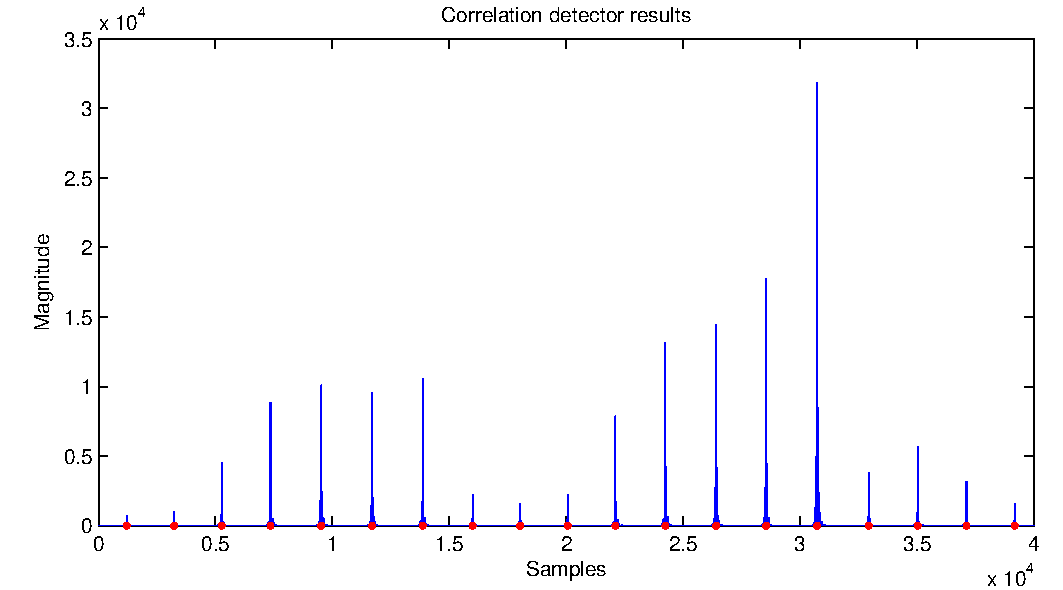
\includegraphics[width=150mm]{correlationDetect.pdf}
\caption{Output of correlation detection code. The red dots indicate detected taps.}\label{fig:correlationDetect}
\end{figure}

With all the taps in the audio stream detected it is now possible to align them for further processing.

\begin{figure}[!]
\centering
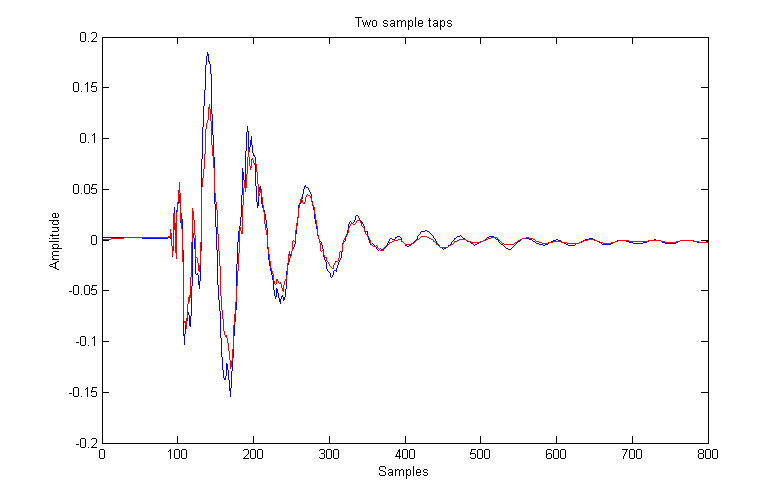
\includegraphics[width=110mm]{twoSampleTaps.png}
\caption{Two taps recorded at the same spot immediately after each other. Sampled at 44.1 kHz.}\label{fig:twoSampleTaps}
\end{figure}

Figure~\ref{fig:twoSampleTaps} shows a modest example of the variability that exist when tapping an object in seemingly the exact same manner. This variability is partly due to noise but bigger variations in the waveform are more likely caused by minute variations in tapping position, intensity and method. In an attempt to obtain a 1 dimensional model that represents a diverse selection of taps at the same spot for the ML and MAP method, the model is constructed as a mean of an ensemble of taps at this position. The mean template is manually trimmed to minimize data size and avoid excessive data that carries no information about the template. Figure~\ref{fig:alignedAndMean} shows a diverse set of aligned taps at a single point in blue and the corresponding mean in red.

\begin{figure}[!]
\centering
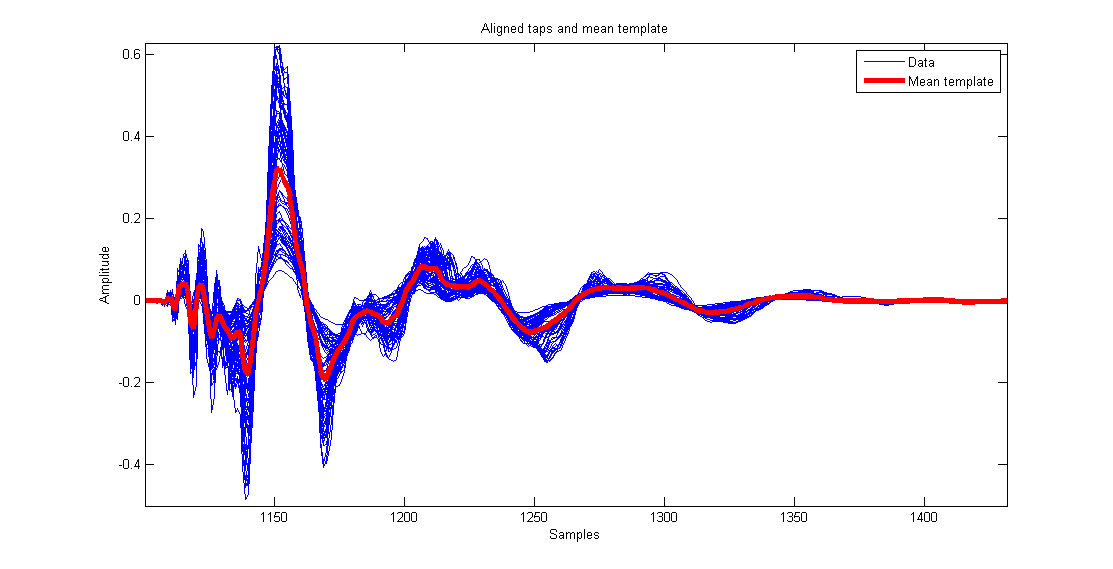
\includegraphics[width=150mm]{alignedAndMean.png}
\caption{Aligned taps with corresponding mean template superimposed on top. Sampled at 44.1 kHz.}\label{fig:alignedAndMean}
\end{figure}

Due to the nature of this algorithm it is essential that it can be executed rapidly and in real time. To accomplish a rapid execution sub-calculations, independent of $y$, from equation (\ref{eq:MLloglikelihood}) has been pre-computed.

The PCA type method requires a different type of template. Here the template is derived via a PCA of the covariance matrix derived from the aligned tapping data as described above.

First the mean and the covariance matrices for each spot $j$ are calculated:

\begin{eqnarray}\nonumber
\mu^j &=& \frac{1}{N^j} \sum_k x^j_k \\\label{eq:PCAcovariance}
C^j &=& \frac{1}{N^j}\sum_k \left(x^j_k - \mu^j\right)\left(x^j_k - \mu^j\right)^T,
\end{eqnarray}
where $x^j_k$ is the $k$th segment of the tapping stream containing a tap on the $j$th spot and $N^j$ is the sample length of the $j$th template. The eigenvalues and the eigenvectors of the covariance matrices $C^j$ are then computed, and the required number of components $q$ (eigenvectors) are chosen based on the corresponding descending values of the eigenvalue. Figure~\ref{fig:eigenvalues} shows an example of a descending order of eigenvalues from an eigenvalue decomposition of the covariance matrix $C^j$.

\begin{figure}[!]
\centering
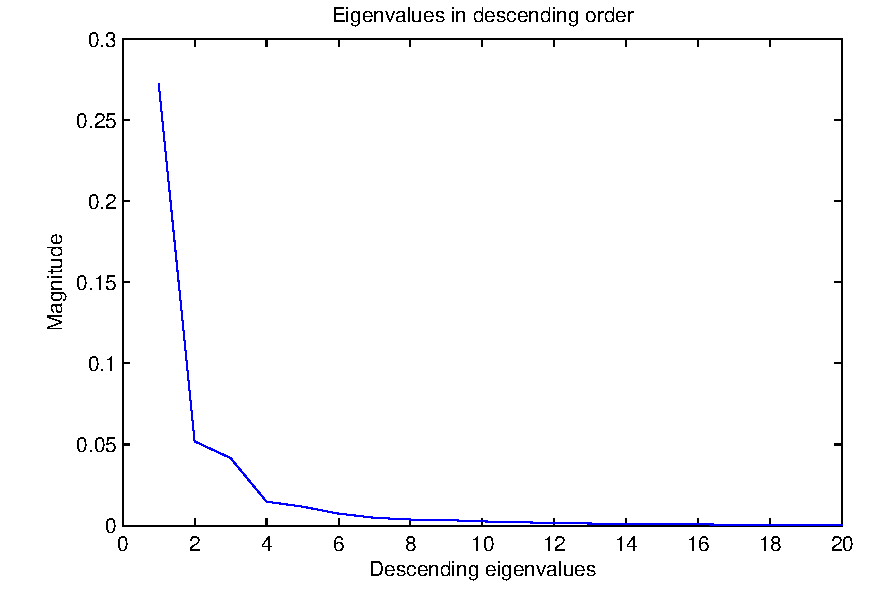
\includegraphics[width=120mm]{eigenvalues.pdf}
\caption{Descending eigenvalues from a eigenvalue decomposition of a covariance matrix $C^j$.}\label{fig:eigenvalues}
\end{figure}

As with the previous method, it is also possible to allocate sub-calculations independent of $y$ from equation~(\ref{eq:z2}) to the training stage to avoid heavy calculations during runtime. In addition, $\mu_\Theta$ is also defined during the training stage.

Figure~\ref{fig:trainingsytemRotate} shows a block diagram of the implementation of the training algorithm. The training data $x^j$ is acquired by the user tapping multiple times on a specific spot $j$. The $N$ taps in this data stream $x^j$ is then detected and aligned with each other as an ensemble in a matrix. Figure~\ref{fig:trainingsytemRotate} shows this as $\textbf{x}^j =  [ x_1^j, x_2^j, \ldots , x_N^j ] $ and as the $N$ taps superimposed on each other in the little plot. From the ensemble the mean $\mu^j$ and the covariance matrix $C^j$ is computed, and from the covariance matrix $C^j$ the eigenvalues and eigenvectors are derived. The $q$ largest eigenvalues are selected and the corresponding eigenvectors are stored as the templates $t^j = [\alpha^j_1,\alpha^j_2,\ldots,\alpha^j_q] $ while the eigenvectors are stored as $C_\Theta^j = diag\{\lambda_1^j,\lambda_2^j,\ldots,\lambda_q^j \}$.

\begin{figure}[!]
\centering
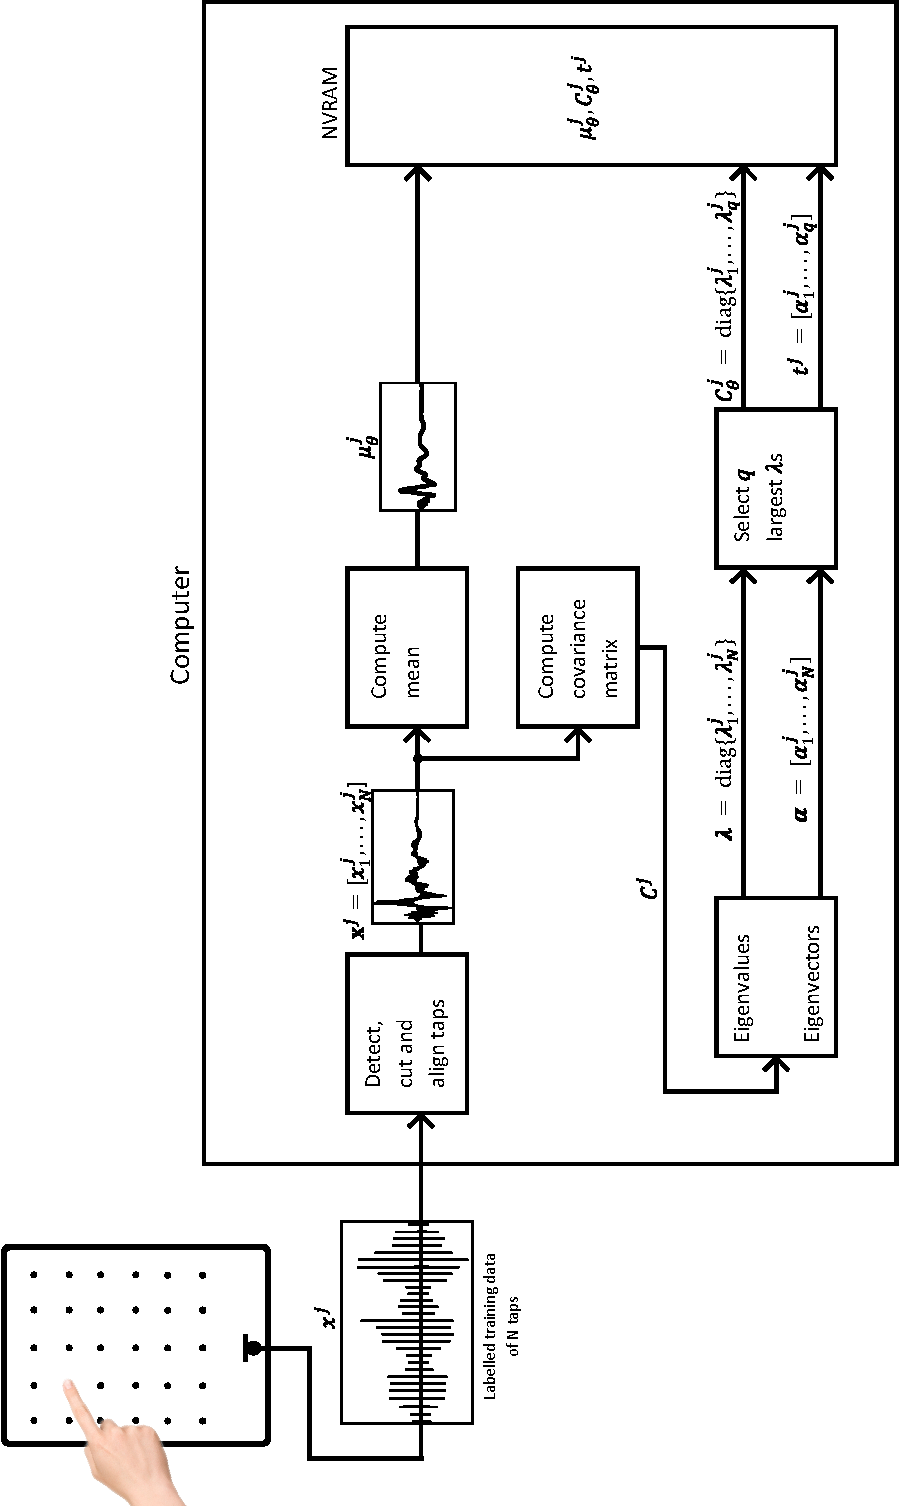
\includegraphics[width=360px]{trainingsytemRotate.pdf}
\caption{Block diagram of training stage of algorithm.}\label{fig:trainingsytemRotate}
\end{figure}

\subsection{Sparse training extension}\label{sec:APRspareTraining}
The methods outlined above requires labeled training data for each model in the classifier. Since this is entirely manageable to obtain this data for low resolution implementation of the pulse recognition system, obtaining this data on a larger device with a greater resolution can become cumbersome and time consuming. This extension of the standard training method for the ML and MAP methods enables detection of points outside the training grid at a scalable resolution.

To achieve this extended resolution, the algorithm creates a linear interpolation between neighboring templates. The assumption is that the acoustic pulses vary relatively linearly between the two templates and hence it may be possible to estimate any template in between the two. Since the mobile phone, used for the previous implementation, undoubtedly is a very complicated vibrational system it was hypothesized that the solid wooden board might provide a more predictable vibrational system and hence a better implementation platform for the interpolation algorithm.

For a number of tapping spots evenly distributed on a line, the interpolated template $t$ at position $x$ along the line on the board can be interpolated by

\begin{equation}\label{eq:interp}
t = t_0 + \left(x - x_0\right) \frac{t_{1} - t^j}{x_1 - x_0},
\end{equation}

where $t_0$ and $t_1$ is the template at the position $x_0$and $x_1$ respectively and $x_0 < x < x_1$.

An example of the a section of the waveforms resulting from this interpolation can be seen in Figure~\ref{fig:InterpData}. Here the thick lines represent the templates computed from data while the thin lines are interpolated templates. The linearly varying color, between red and black of the thin lines, shows the relative distance of the template position $x$ in this example.

\begin{figure}[!]
\centering
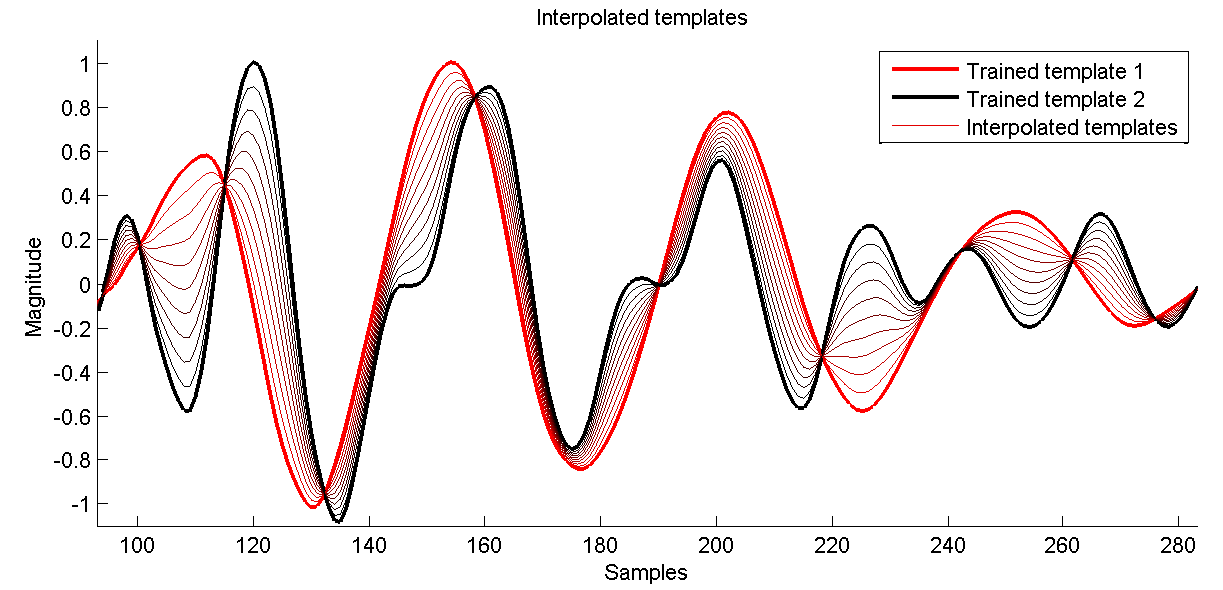
\includegraphics[width=360px]{InterpData.pdf}
\caption{Example of section of a interpolated waveforms using linear interpolation.}\label{fig:InterpData}
\end{figure}

To achieve a full 2D grid of interpolated templates amongst templates derive from data, requires a second round of interpolation in the second dimension for each column.

While the assumption of linearly changing pulses might be valid, it is still necessary to align the neighboring templates accurately. Aligning taps accurately has proven difficult with the correlation method due to the change in the pulses over the surface of the board. To provide a more accurate alignment method a second microphone was attached to the stylus while tapping to provide a consistent reference tap. The idea was that this consistent tap should provide exact alignment between all the taps. Figure~\ref{fig:templatesAligned} shows the result of this alignment.

\begin{figure}[!]
\centering
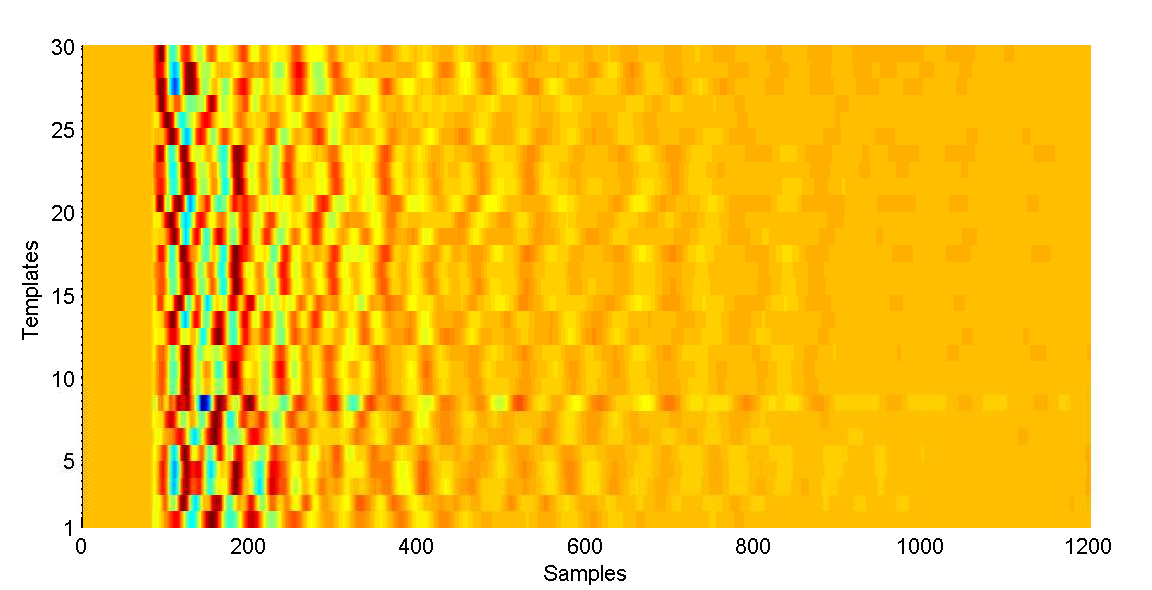
\includegraphics[width=380px]{templatesAligned.pdf}
\caption{30 templates from wooden board aligned. Seen from above.}\label{fig:templatesAligned}
\end{figure}

The benefit of a representation like Figure~\ref{fig:templatesAligned} is that since the wooden board is laid out in a grid of 6 by 5 spots, spot numbering starting in top left corner and following reading direction, Figure~\ref{fig:templatesAligned} allows for assessment of alignment row by row.

The standard 6 by 5 spot resolution on the wooden board can be expanded to 51 by 41 spots simply by interpolating 9 templates between each trained spot row-wise and then doing the same for all 41 columns. The running of the detection algorithm will proceed as before although at a substantially slower rate.

\section{Results}\label{sec:results}
In this section the empirical evaluations of the methods mentioned above will be presented. To test the algorithms, two sets of data is needed; a training set $D^1$ and a testing set $D^2$. The training set is used in the training stage of the algorithm, as mentioned above, and the testing data is essentially the data that the algorithm attempts to model and classify. In an attempt to evaluate the algorithms' robustness to variations, two different sets of training and testing data is used. One set is recorded using a stylus to tap on the device, $D^1_S$ and $D^2_S$, and the second set is tapped using a finger nail, $D^1_N$ and $D^2_N$. Although it might be informative to use the same data for the training and testing stage, in this test the two sets are independently recorded, in identical conditions, which means that there in total are 4 data sets $D^1_S$, $D^2_S$, $D^1_N$ and $D^2_N$, which will be used to test the algorithms in various combinations to give a picture of the performance of the algorithms.

\begin{figure}[!]
\centering
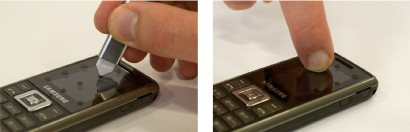
\includegraphics[width=410 px]{tapSN.png}
\caption{To the left is an example of a tap with the stylus and to the right a tap with a fingernail.}\label{fig:tapSN}
\end{figure}

 Each set of training data contains approximately 70 taps at each spot on the device totalling approximately $70 \times 12 = 840$ taps tapped with varying force. To estimate the performance of the algorithm given certain criteria there are 3 outcomes of a test. The tap may be correctly classified, misclassified (classified as any of the 11 other spots) or it may avoid detection entirely and hence be classified as a missed detection $j=0$. The ratio of these 3 outcomes may vary with a large number of parameters within the algorithm such as various thresholds for detection or classification, template length, filtering or number of PCs used under training, so the performance of the algorithm will always be presented in relation to a varying parameter. It is worth noting that all data used in the production of these results have been high-pass filtered at with a cut-off frequency of 441 Hz. The effect of this filtering has not exhaustively been investigated, but provides visually a ``cleaner'' signal, and does not appear to harm the performance.

Figure~\ref{fig:PCAperform} shows the performance of the PCA type algorithm using the training data $D^1_S$ and the testing data $D^2_S$. The figure gives an idea of how the performance changes with changing number of components $q$ used in the templates. Figure~\ref{fig:PCAperform} clearly shows that the rate of correct classification is beyond 90\% down to 2 components whereafter it drops of sharply to below 10 \%. It is noted that the performance drops to around 8\% which is exactly what would be expected by a random guess or the prior knowledge $p(j)= \frac{1}{J}$. A decrease in performance is detectable from 4 components and down, whereas the performance for 5 components and more appears constant.

\begin{figure}[!] %PCA components S-S
\centering
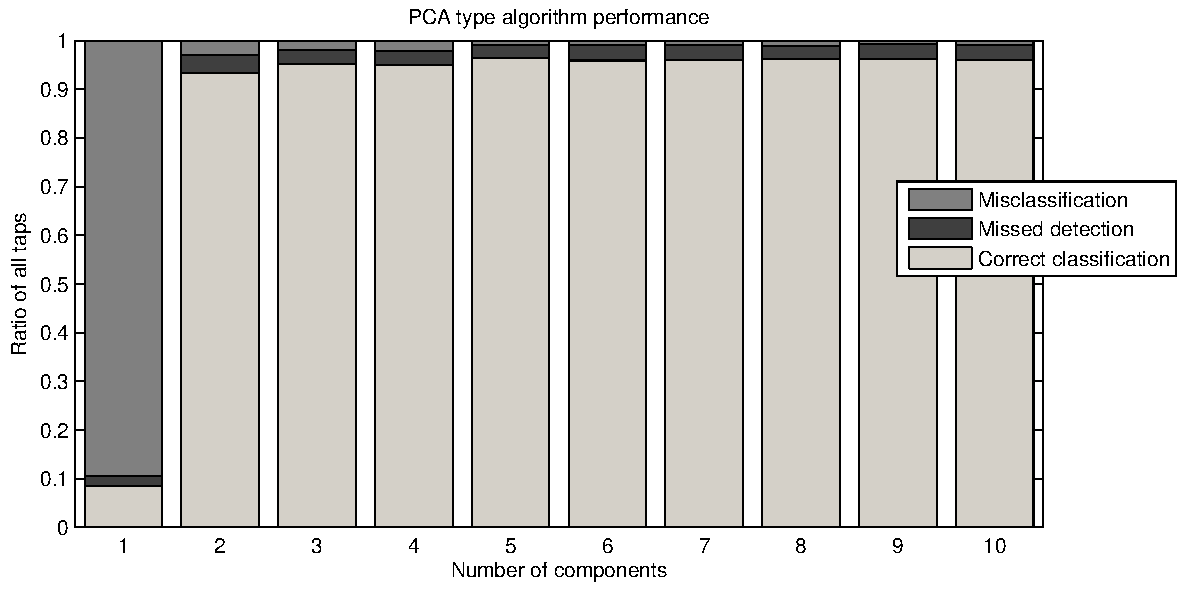
\includegraphics[width=150mm]{PCAperform.pdf}
\caption{Performance of the PCA type algorithm for different numbers of PCA components and with a template length $M=250$ samples. Training data: $D^1_S$, Testing data: $D^2_S$.}\label{fig:PCAperform}
\end{figure}

In Figure~\ref{fig:PCAperformLength} the relation between performance and template length $M$ can be seen with a test conducted with the same data as the previous. The performance of the algorithm appears unaffected by $M$ at template lengths above 150 samples although for $M<150$ the performance decreases dramatically and as with Figure~\ref{fig:PCAperform} appears to settle around $p(j)$. The ratio between missed detections and misclassifications appear to vary greatly at low values for $M$ and it is currently not certain why this occurs but it is worth mentioning that this ratio is purely determined by a threshold in the algorithm and can be fine tuned for desired outcome.

\begin{figure}[!] %PCA length S-S
\centering
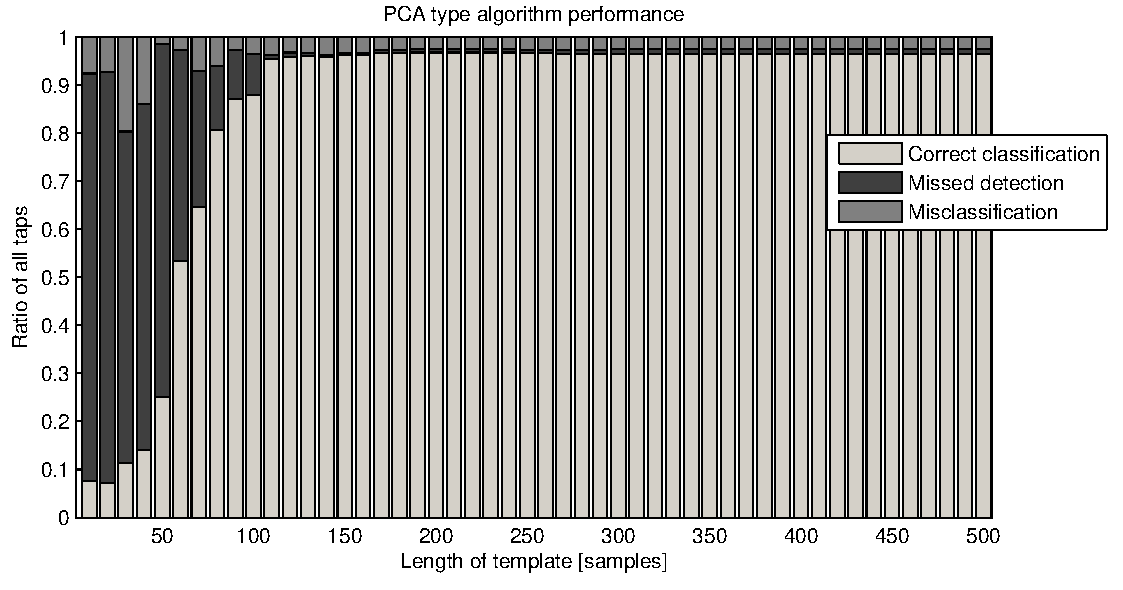
\includegraphics[width=150mm]{PCAperformLength.pdf}
\caption{Performance of the PCA type algorithm for different values of template length $M$ for components $q=5$. Training data: $D^1_S$, Testing data: $D^2_S$,}\label{fig:PCAperformLength}
\end{figure}

Figure~\ref{fig:MLperform} shows the performance of the ML based algorithm using training data $D^1_S$ and testing data $D^2_S$. This figure shows the effect of changing the template length $M$ on the detection performance. As in Figure~\ref{fig:PCAperformLength} the performance appears to peak and stay constant at $M>150$ and for $M<50$ the performance appears equally unaffected and as with the PCA algorithm appears to approach the prior probability of detection which in this case is set as being uniform across the different spots $j$.

Another feature of Figure~\ref{fig:MLperform} is the ratio of various detection results. Whereas the PCA type algorithm replaced correct classifications with misclassifications when the number of components fell below 5, the ML algorithm appears to miss the detection of the tap entirely. This difference in the two methods is caused by a difference in the threshold for a missed detection.


\begin{figure}[!] %ML length S-S
\centering
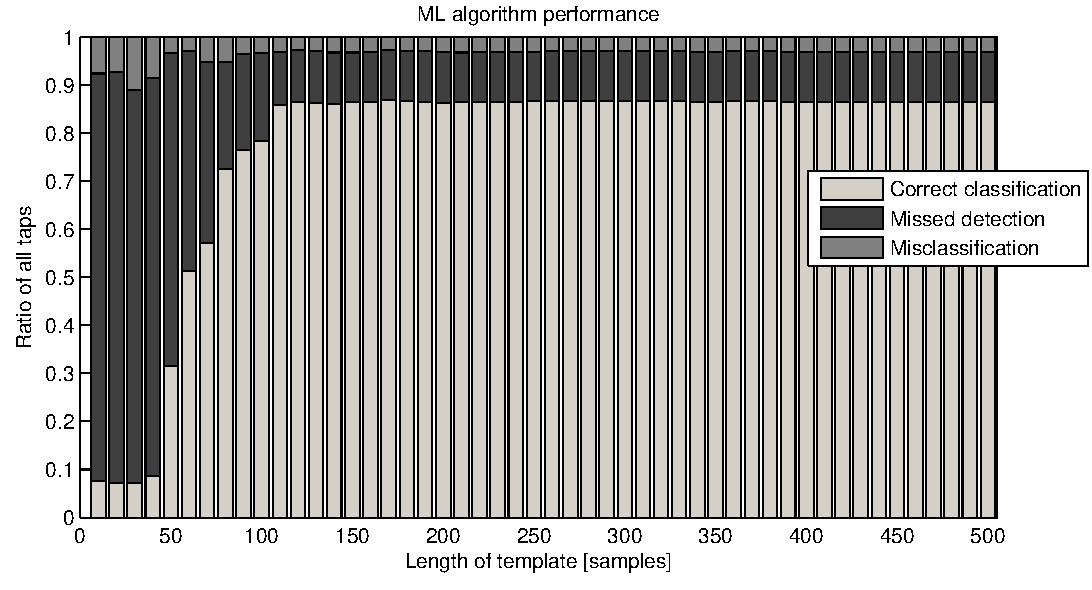
\includegraphics[width=150mm]{MLperform.pdf}
\caption{Performance of the ML algorithm for different template sample lengths $M$ for components $q=5$. Training data: $D^1_S$, Testing data: $D^2_S$.}\label{fig:MLperform}
\end{figure}

For completeness Figure~\ref{fig:MAPperformLength} has been included to show the performance of the MAP algorithm. The training and testing set up is identical to the previous evaluation of the ML algorithm and the performance appears to be almost identical.

\begin{figure}[!] %MAP Length S-S
\centering
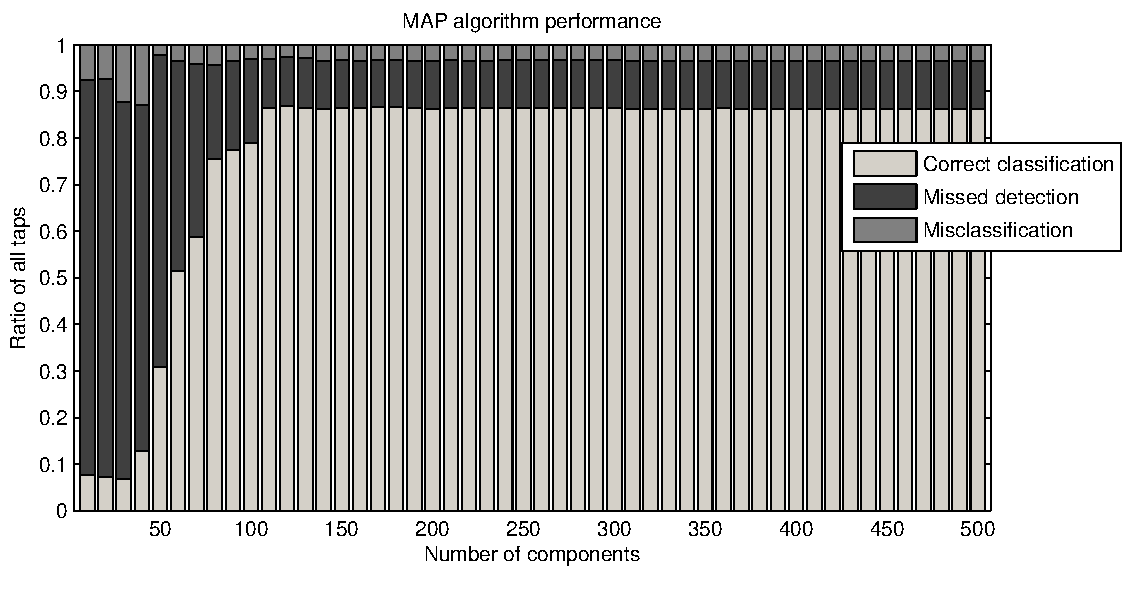
\includegraphics[width=150mm]{MAPperformLength.pdf}
\caption{Performance of the MAP algorithm for different template sample lengths $M$ for components $q=5$. Training data: $D^1_S$, Testing data: $D^2_S$.}\label{fig:MAPperformLength}
\end{figure}

Figure~\ref{fig:PCAperformNail} shows the performance of the PCA type algorithm with $q$ again varying from 1 to 10, with training data $D^1_S$ and testing data $D^2_N$. In other words, the algorithm is tested by tapping using a finger nail but trained using only a stylus. This test is conducted to evaluate the PCA type algorithms ability to cope with testing data significantly different to the training data, and more specifically to evaluate the effect on the performance in relation to the number of components included $q$. The figure shows a significantly reduced performance although the performance in relation to $q$ appears similar. For $q=1$ the performance still approaches $p(j)$.

\begin{figure}[!] %PCA components S-N
\centering
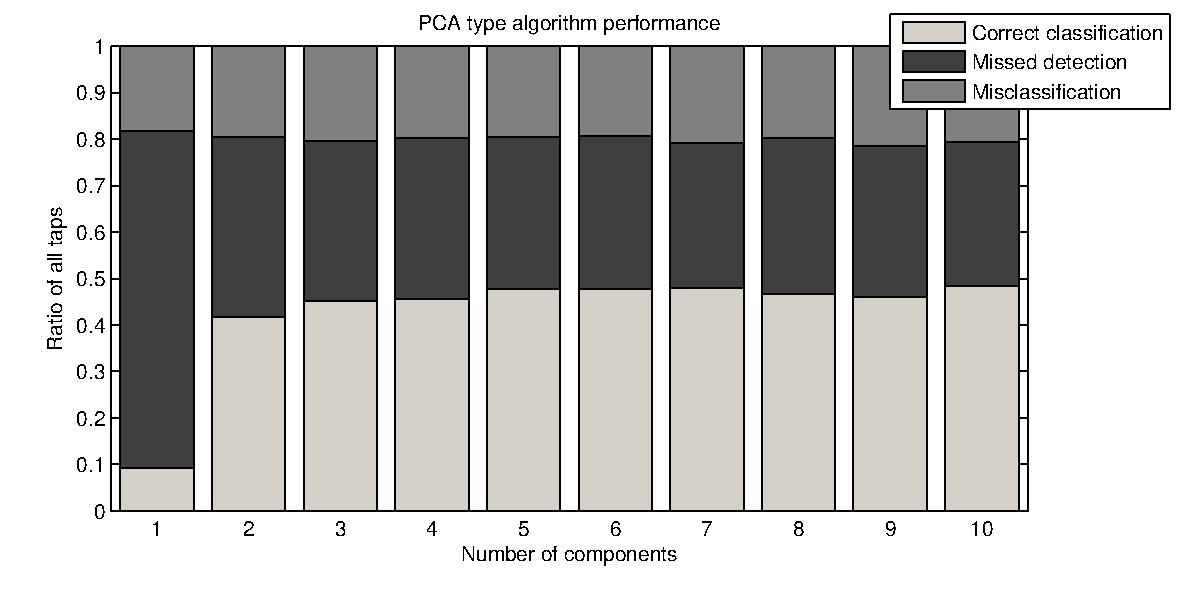
\includegraphics[width=150mm]{PCAperformNail.pdf}
\caption{Performance of the PCA type algorithm for different numbers of PCA components and with a template length of $M=250$ samples. Data used to evaluate performance was tapped using finger nails rather than the stylus used for training. Training data: $D^1_S$, Testing data: $D^2_N$.}\label{fig:PCAperformNail}
\end{figure}

The motivation for developing the PCA type algorithm was to be able to model data with a high degree of variability. Figure~\ref{fig:PCAperform_SN-SN} shows the performance of the PCA type algorithm in relation to changing $q$ with training being done with both the stylus $D^1_S$ and finger nail data $D^1_N$. By training on both sets it was hypothesized that the increased variability in the training data would be mirrored in the components, enabling the algorithm to cope with an equally increased degree of variability during the testing stage. To simulate the increased variability during the testing stage this test was conducted using stylus $D^2_S$ and finger nail $D^2_N$ data as well.

\begin{figure}[!] %PCA components SN-SN
\centering
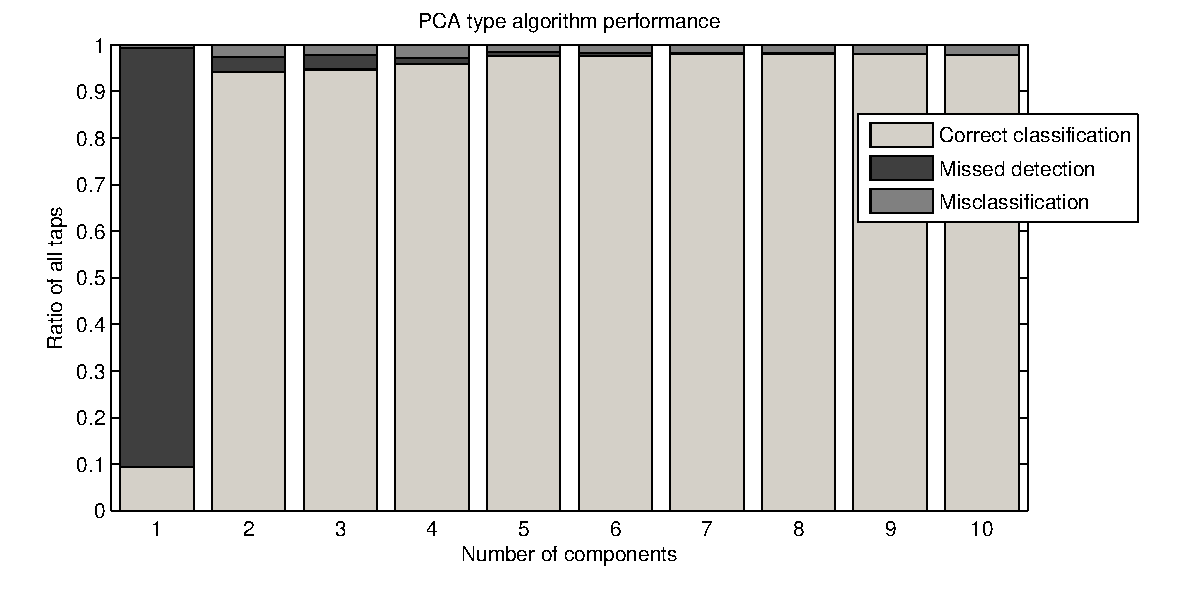
\includegraphics[width=150mm]{PCAperform_SN-SN.pdf}
\caption{Performance of the PCA type algorithm for different numbers of PCA components and with a template length $M=250$ samples. Training data: $D^1_S$ and $D^1_N$, Testing data: $D^2_S$ and $D^2_N$}\label{fig:PCAperform_SN-SN}
\end{figure}

Figure~\ref{fig:PCAMLMAPperform} gives an overview of the performance of the different algorithms with various data sets being used for testing and training. The specific data used for each test is noted on the figure itself. Please note that for all tests in Figure~\ref{fig:PCAMLMAPperform}, $M=250$ and $q=5$. These values have been determined as sufficient in the tests above.

\begin{figure}[!] %PCA-ML-MAP compare
\centering
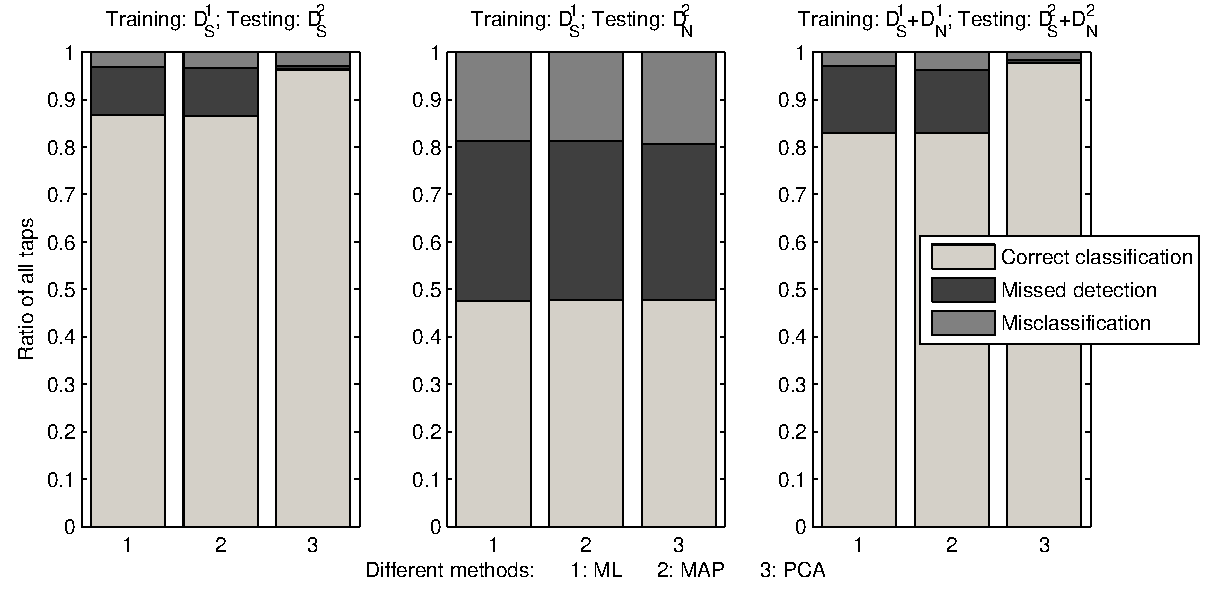
\includegraphics[width=150mm]{PCAMLMAPperform.pdf}
\caption{Performance of all 3 algorithms in 3 different tests. All tests conducted with $M=250$ and $q=5$. $D^1_S + D^1_N$ refers to two sets of data being merged together, not added.}\label{fig:PCAMLMAPperform}
\begin{picture}(0,0)
\put(-200,260){a)}
\put(-74,260){b)}
\put(55,260){c)}
\end{picture}
\end{figure}

A selected run of the sparse training extension, for the ML algorithm, has given a result presented in Figure~\ref{fig:padPlot}. The intensity map shows the highest probability near the spot actually tapped, which is between spot 7 and 8. Figure~\ref{fig:padPlot} also reveals other areas of high probability. It is stressed that this run is a selected run of the algorithm and the performance is not consistently of this standard, although the Figure~\ref{fig:padPlot} does provide a good representation of the algorithm when it is working, with several areas of high probability being a common feature.

\begin{figure}[!]
\centering
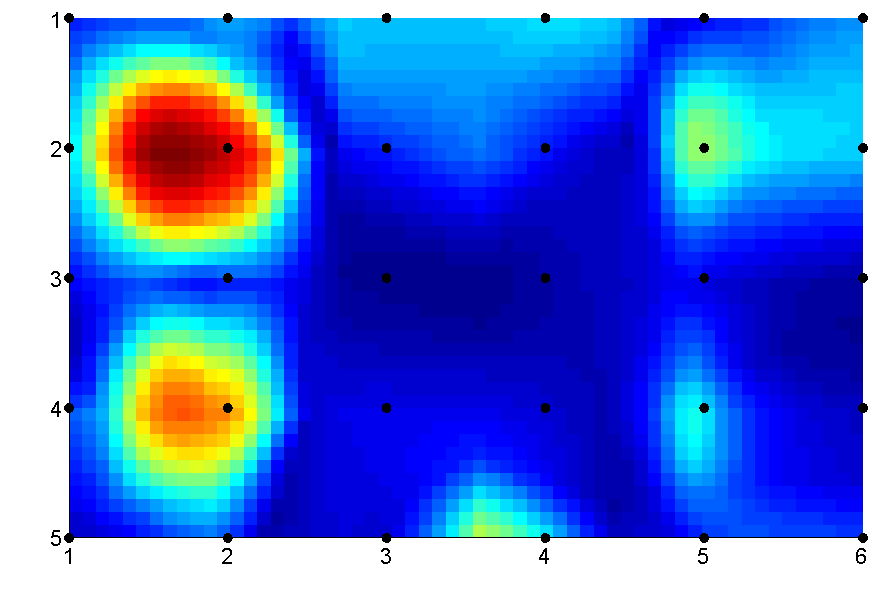
\includegraphics[width=150mm]{padPlot.pdf}
\caption{Intensity map of model probabilities. Black dots represent trained tapping spots, as seen on Figure~\ref{fig:Pad}. }\label{fig:padPlot}
\end{figure}

\section{Discussion}

The results from the previous section enables one to make a range of assertions about the relative performance of the different algorithms in various conditions. It is for example noticed in Figure~\ref{fig:PCAperform}, \ref{fig:PCAperformNail} and \ref{fig:PCAMLMAPperform} that the performance of the PCA varies greatly by including 2 rather than 1 components in the template set. It is also noted from Figure~\ref{fig:PCAperform} and \ref{fig:MLperform} that with only 2 components, $q=2$, the PCA easily outperforms the ML (and MAP) method but with only 1 component, $q=1$, the performance of the PCA drops to $p(j)$. Although both the ML and PCA are equivalent from the viewpoint of the detection for $q=1$, it is clear that there performance is not. In the case of $q=1$ what separates the two algorithms are how the template $t^j(n_0)$ is derived. It appears that the mean template is more effective in classifying pulses than the PC is. The most likely explanation for this behavior is that the PC of one of the taps is a sufficiently broad interpretation of the tap that it results in a high likelihood in each case and hence ``wins'' each classification. This hypothesis is further supported by the performance for $q=1$ in Figure~\ref{fig:PCAperform_SN-SN}, where the ratio between missed detections and misclassifications is entirely different with an overwhelming number of missed detections to misclassifications. In this case, with this training data, the PC was clearly a much less likely fit to the testing data.

Figures~\ref{fig:PCAperformLength}, \ref{fig:MLperform} and \ref{fig:MAPperformLength} consistently suggest that the performance of all algorithms appear almost unaffected of template length $M$ for lengths $M\geq110$. The PCA algorithm performance appear to have a slight gradient up to $M=170$, although this might simply be due to the trimming of the aligned taps for one of the templates. Besides this slight difference, the change of template length $M$ appears to affect all methods in a similar manner.

The PCA type algorithm was derived with the intention of creating a model being able to cope with a higher degree of variability than the ML and MAP methods. Although Figure~\ref{fig:PCAperformNail} shows relatively poor performance for different testing data to training data, it is worth noting that when the algorithm is allowed to train with data of higher variability, see Figure~\ref{fig:PCAperform_SN-SN}, a dramatic improvement is seen. This performance boost appears to even outperform the PCA with no merged data, see Figure~\ref{fig:PCAperform}, which might be explained by the increased training data allows the derived components to be more robust to even minor variability that potentially could ``confuse'' the PCA otherwise.

Figure~\ref{fig:PCAMLMAPperform} gives a definitive insight into the relative performance between all the algorithms in various conditions, and it is clear that the PCA algorithm has a significant performance edge, specifically when it comes to testing data with greater variability. Comparing graph a and c in Figure~\ref{fig:PCAMLMAPperform} it is seen that the greater variability in the testing data affects the methods that use a mean template negatively. The increased variability results in mean templates that focus on some broader aspects of the data and more subtle variations are lost. It is although again noticed that the PCA method performs better under these circumstances.

Although no quantifiable results of the performance of the interpolated training algorithm exist, preliminary tests show that the system is able to detect some off- grid points with relative success in certain very specific regions of the board, but for the most part the results are fairly random. It is thought that this performance is due to problems with either alignment or more erratic and unpredictable pulses arising from certain regions. The common feature of multiple high probability regions observed in Figure~\ref{fig:padPlot} is more than likely due to symmetry in the mechanical structure being reflected in the vibrational characteristics of the device. The issue of the structural symmetry is thought to specifically be an issue on the wooden board due to its mechanical uniformity, although the intensity map does generally show the correct tapping position with higher probabilities than the other peaks created by symmetry.

\section{Conclusions}

The algorithms presented in this report as part of the first year of the PhD, has shown promising performance. The multi-component approach to the classification algorithm has shown to provide robustness in light of uncertainty in the use of tapping tools and in fact provide better performance if allowed to train on varied data. The multi-component approach to acoustic pulse recognition has consistently outperformed the ML and MAP methods also presented in this report.

A range of possible extensions to the models and algorithms have been identified in the literature, and new ideas and extensions have been outlined and included in the time plan for the further research. Further studies into the nature of the variations observed in tapping data will provide further inspiration on extensions combined with the extensions outlined in the time plan should provide a suitable PhD project.

\subsection{Possible future work}

% ------------------------------------------------------------------------


%%% Local Variables:
%%% mode: latex
%%% TeX-master: "../thesis"
%%% End: 